\documentclass[12pt, a4paper, titlepage]{article}

\usepackage[a4paper, includeheadfoot, margin=2.54cm]{geometry}
\usepackage{graphicx}
\usepackage[dvipsnames]{xcolor}
\usepackage{sectsty}
\usepackage{titling}
\usepackage{fancyhdr}
\usepackage{pgfplots}
\usepackage{tikz}
\usepackage{tikz-3dplot}
\usetikzlibrary{arrows.meta}
\usetikzlibrary{shapes.geometric, arrows}
\usepackage{mathtools}
%\usepackage[ngerman]{babel}
\usepackage[utf8]{inputenc}
\usepackage{paralist}
\usepackage{color}
\usepackage{eso-pic}
\usepackage{wrapfig}
\usepackage{amssymb}
\usepackage{chemfig}
\usepackage{multirow}
\usepackage{array}
\usepackage{multicol}
\usepackage{calc}
\usepackage{ragged2e}
\usepackage{mathtools}
\usepackage{empheq}
\usepackage{colortbl}
\usepackage{pifont}
\usepackage{savesym}
\usepackage{marvosym}
\usepackage{braket}
\usepackage{anyfontsize}
\usepackage{listings}
\usepackage{makecell}
\usepackage{svg}
\usepackage{mdframed}
\usepackage{extarrows}
\PassOptionsToPackage{obeyspaces}{url}
\usepackage[pdftex, pdfauthor={Philipp A. Huber}, pdftitle={The Bible of Physics}, colorlinks,
pdfpagelabels,
pdfstartview = FitH,
bookmarksopen = true,
bookmarksnumbered = true,
linkcolor = black,
plainpages = false,
hypertexnames = false,
citecolor = black, urlcolor=black] {hyperref}


%Dokumenteinstellungen
\definecolor{myblue}{RGB}{212,217,255}
\definecolor{myblue2}{RGB}{40,40,115}
\definecolor{myblack}{RGB}{14,14,14}
\definecolor{mygrey}{RGB}{240,240,240}
\pagestyle{fancy}
\lhead{HPC}
\rhead{Unix Commands}
\chead{Philipp Huber (14-936-694)}
\cfoot{\thepage}
\setcounter{secnumdepth}{0}
\tikzstyle{block} = [rectangle, minimum width = 4cm, minimum height = 1cm, fill = myblue, text centered]
\tikzstyle{gblock} = [rectangle, minimum width = 4cm, minimum height = 1cm, fill = mygrey, text centered]
\tikzstyle{arrow} = [thick,->,>=stealth]
\tikzstyle{tarrow} = [very thick,->,>=stealth]
\tikzstyle{uarrow} = [ultra thick,->,>=stealth]
\setlength\parindent{0pt}
\lstset{basicstyle=\ttfamily\small,breaklines=true}
%\partfont{\color{myblue2}} 
%\sectionfont{\color{myblue2}} 
%\subsectionfont{\color{myblue2}}


%New Commands
\newcommand{\bx}[1]{
    \begin{center}
  	    \fboxrule2mm
	    \fcolorbox{myblue}{myblue}{
	    \begin{math}
	    #1
        \end{math}
        }
    \end{center}
}

\newcommand{\bbx}[1]{
	    \begin{mdframed}[backgroundcolor=myblue, innertopmargin=10pt, innerbottommargin=10pt, topline=false, bottomline=false, rightline=false, leftline=false]
	    #1
    \end{mdframed}
}

\newcommand{\gbx}[1]{
	    \begin{mdframed}[backgroundcolor=mygrey, innertopmargin=10pt, innerbottommargin=10pt, topline=false, bottomline=false, rightline=false, leftline=false]
	    #1
    \end{mdframed}
}        


\newcommand{\wbx}[1]{
    \begin{center}
        \fboxrule2mm
	    \fcolorbox{white}{white}{
	    \begin{math}
	    #1
        \end{math}
        }
    \end{center}
}
\newcommand{\myref}[2]{\hyperref[#2]{\textcolor{myblue2}{\MVRightarrow} \hspace{-0.1cm}\textit{#1}} (Seite \pageref{#2})}
\newcommand{\tocref}[2]{\hyperref[#2]{\textcolor{myblue2}{\MVRightarrow} \hspace{-0.1cm}\textsc{#1}}}
\newcommand{\cd}{\cdot}
\renewcommand{\arraystretch}{1.5}
\newcommand{\abl}{\text{d}}
\newcounter{def}
\newcounter{bsp}
\newcounter{anl}
\newcommand{\defi}[1]{\textbf{Definition \stepcounter{def}\arabic{def}} \textbf{(#1)}}
\newcommand{\bsp}{\textbf{Beispiel \stepcounter{bsp}\arabic{bsp}} }
\newcommand{\anl}{\textbf{Anleitung \stepcounter{anl}\arabic{anl}} }
\newcommand{\R}{\mathbb{R}}
\newcommand{\C}{\mathbb{C}}
\newcommand{\N}{\mathbb{N}}
\newcounter{src}
\newcommand{\src}[1]{\stepcounter{src}\expandafter\xdef\csname#1\endcsname {\arabic{src}}\hyperref[Quellenverzeichnis]{[\arabic{src}]}}
\newcommand{\iql}[4]{#1$\quad$#2: \url{#3} (#4)}
\newcommand{\itm}{\item[\tiny\color{myblue2}\ding{110}]}
\newcommand{\formel}[1]{\vspace{0.3cm}
\begin{gather*}
	#1
\end{gather*}\par
\vspace{0.3cm}
\noindent}
%\expandafter\def\expandafter\UrlBreaks\expandafter{\UrlBreaks}%  save the current one
%  {\do\a\do\b\do\c\do\d\do\e\do\f\do\g\do\h\do\i\do\j%
%  \do\k\do\l\do\m\do\n\do\o\do\p\do\q\do\r\do\s\do\t%
%  \do\u\do\v\do\w\do\x\do\y\do\z\do\A\do\B\do\C\do\D%
%  \do\E\do\F\do\G\do\H\do\I\do\J\do\K\do\L\do\M\do\N%
%  \do\O\do\P\do\Q\do\R\do\S\do\T\do\U\do\V\do\W\do\X%
%  \do\Y\do\Z}
\newcommand{\bibspace}{\hspace*{0.83cm}}
\newcommand{\vp}{\vspace{1cm}}
\newcommand{\der}{\text{d}}













%%%%%%%%%%%%%%%%%%%%%%%%%%%%%%%%%%%%%%%%%%%%%%%%%%%%%%%%%%%%%%%%%%%%%%%%%%%%%%%%%%%%%%%%%%%%%%%%%%%%%%%%%%%%%%%%%%%%%%%%%%%%%%%%%%%%%%%%%%%%%%%%%%%%%%%%%%%%%%%%%%%%%%%%%%%%%%%%%%%%%%%%%%%%%%%%%%%%%%%%%%%%%%%%%%%%%%%%%%%%%%%%%%%%%%%%%%%%%%%%%%%%%%%%%%%%%%%%%%%%%%%%









%Dokumentbeginn
\begin{document}

\lstset{language=Fortran}




%Titelseite
\begin{titlepage}
	\enlargethispage{1cm}
	\color{white}
	\vspace*{1cm}
	\tikz[remember picture, overlay] \node[opacity=0.9, below=0cm] at (current page.north)      {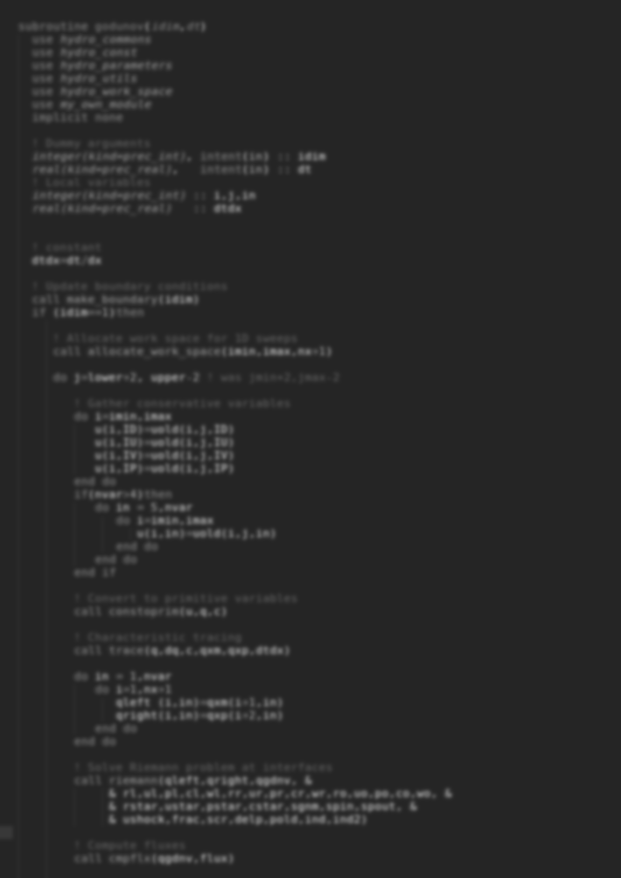
\includegraphics[width=21.40cm]{pictures/code2.png}};	
    \begin{tikzpicture}[remember picture, overlay]
    \node (A)  at (current page.south west) {};
    \node (B)  at (current page.north west) {};
    \node (C)  at (current page.north east) {};
    \node (D)  at (current page.south east) {};
    \coordinate (cA) at (A) ;
    \coordinate (cB) at (B);
    \coordinate (cC) at (C);
    \coordinate (cD) at (D) ;
    \draw[line width=6mm] (cA) -- (cB) -- (cC) -- (cD) -- cycle;
    \node[white, left] at (16, -3) {\sffamily \fontsize {33}{33} \selectfont Parallelizing The Hydro Code};
    \node[white, left] at (16, -5.15) {\sffamily \fontsize{23}{23}\selectfont Hannes Imboden, Philipp A. Huber};
    \node[white, left] at (16, -9) {\sffamily \fontsize{18}{18}\selectfont High Performance Computing};
    \node[white, left] at (16, -10) {\sffamily \fontsize{18}{18}\selectfont Final Project};
    \node[white, left] at (16, -11) {\sffamily \fontsize{18}{18}\selectfont June 2018};
    \end{tikzpicture}
\end{titlepage}


%\begin{titlepage}
%	\enlargethispage{1cm}
%	\color{white}
%	\vspace*{1cm}
%	\tikz[remember picture, overlay] \node[opacity=0.9, below=0cm] at (current page.north)      {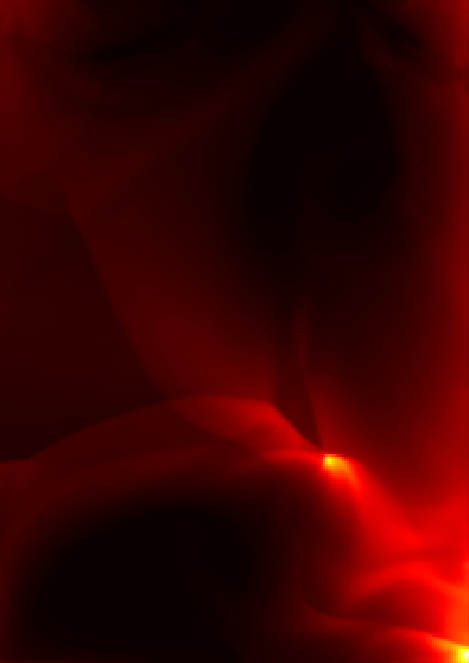
\includegraphics[width=21.40cm]{pictures/hydro2.png}};	
%    \begin{tikzpicture}[remember picture, overlay]
%    \node (A)  at (current page.south west) {};
%    \node (B)  at (current page.north west) {};
%    \node (C)  at (current page.north east) {};
%    \node (D)  at (current page.south east) {};
%    \coordinate (cA) at (A) ;
%    \coordinate (cB) at (B);
%    \coordinate (cC) at (C);
%    \coordinate (cD) at (D) ;
%    \draw[line width=6mm] (cA) -- (cB) -- (cC) -- (cD) -- cycle;
%    \node[white, right] at (-0.15, -3) {\sffamily \fontsize {33}{33} \selectfont Parallelizing the Hydro Code};
%    \node[white, right] at (0, -5) {\sffamily \fontsize{23}{23}\selectfont Hannes F. Imboden, Philipp A. Huber};
%    \node[white, right] at (0, -10) {\sffamily \fontsize{18}{18}\selectfont High Performance Computing};
%    \node[white, right] at (0, -11) {\sffamily \fontsize{18}{18}\selectfont Final Project};
%    \node[white, right] at (0, -12) {\sffamily \fontsize{18}{18}\selectfont June 2018};
%    \end{tikzpicture}
%\end{titlepage}


\newpage
%Contents
\clearpage
\thispagestyle{plain}
\pagenumbering{Roman}
\setcounter{page}{1}
{\pagestyle{plain}
\tableofcontents\label{toc}
\clearpage
\pagenumbering{arabic}
\setcounter{page}{1}
%\thispagestyle{plain}}
%\begingroup
%\let\clearpage\relax
%\listoffigures
%\endgroup
%\begingroup
%\let\clearpage\relax
%\listoftables
%\endgroup




\newpage
\section{Hydro Code Explained}

The hydro code is a simulation of a fluid or gas in an enclosed system. The initial conditions are set as to generate an unperturbed, homogeneous environment. Then, one can introduce points of higher or lower pressure or density to imitate an explosion or jet. The code then calculates the propagation of this perturbation using Godunov's method and outputs each frame as a single file, which can be used to create an animation.\\
%The method used to calculate the dynamics of the fluid is the Godunov's.

There are five main components with different functionality to this Fortran based code. They are:
\begin{itemize}
	\item \texttt{main.f90}
	\begin{itemize}
		\item calls \texttt{init\_hydro} to initialize the grid with the initial conditions
		\item executes the main time loop by calling
		\begin{itemize}
		\item \texttt{output} to generate output data
		\item \texttt{cmpdt} to compute the time step
		\item \texttt{godunov} to calculate the fluid dynamics
		\end{itemize}
	\end{itemize}
	\item \texttt{module\_hydro\_principal.f90} contains the subroutines
	\begin{itemize}
		\item \texttt{init\_hydro}
		\item \texttt{cmpdt}
		\item \texttt{godunov} which calls
		\begin{itemize}
				\item \texttt{make\_boundary} to set the upper, lower, left and right boundaries of the grid
				\item \texttt{allocate\_work\_space}/\texttt{deallocate\_work\_space} to (de)allocate space in the memory
				\item other subroutines for calculation purposes
			
		\end{itemize}
	\end{itemize}
	\item \texttt{module\_hydro\_utils.f90} contains
	\begin{itemize}
		\item \texttt{make\_boundary}
		\item other subroutines
	\end{itemize}
	\item \texttt{module\_hydro\_IO.f90} contains the subroutines
	\begin{itemize}
		\item \texttt{read\_params} to read the parameters from the \texttt{input.nml} file
		\item \texttt{output}
	\end{itemize}
	\item \texttt{module\_hydro\_commun.f90} contains 
	\begin{itemize}
		\item \texttt{allocate\_work\_space}/\texttt{deallocate\_work\_space}
		\item various other subroutines, mainly to define the variables used elsewhere in the code
	\end{itemize}		
\end{itemize}

Additionally, there are several input files to set the grid size, initial condictions, etc.








\section{Parallelization Techniques}
\subsection{MPI}

\subsubsection{Introduction}
MPI stands for \textit{message passing interface}. This refers to the fact that parallel computing occupies multiple CPUs to fasten up the execution of a code. As these CPUs work independently and with their own associated memory, they will have to communicate in some way; this is what MPI does.\\
The advantage of MPI over other libraries is that one has much more control over how the code is parallelized. The programmer can explicitly choose how the different cores communicate to each other and which information they share.\\
On the other hand, this freedom makes parallelizing a code a much more complex problem than it could be with other libraires. It requires quite a deep understanding of how the code works to know where and what to adjust. test


\subsubsection{Parallelization Process}
The main points that needed to be adjusted were the following:

\begin{itemize}
\item Workspace allocation
\item Time step computation
\item Godunov boundaries
\item Communication between boundaries
\item Output formatting
\end{itemize} 


\subsubsection{Results}

The plots for the respective runtimes of both the strong and weak scaling can be seen below:
\begin{figure}[htbp]
	\begin{minipage}{0.49\textwidth} 
	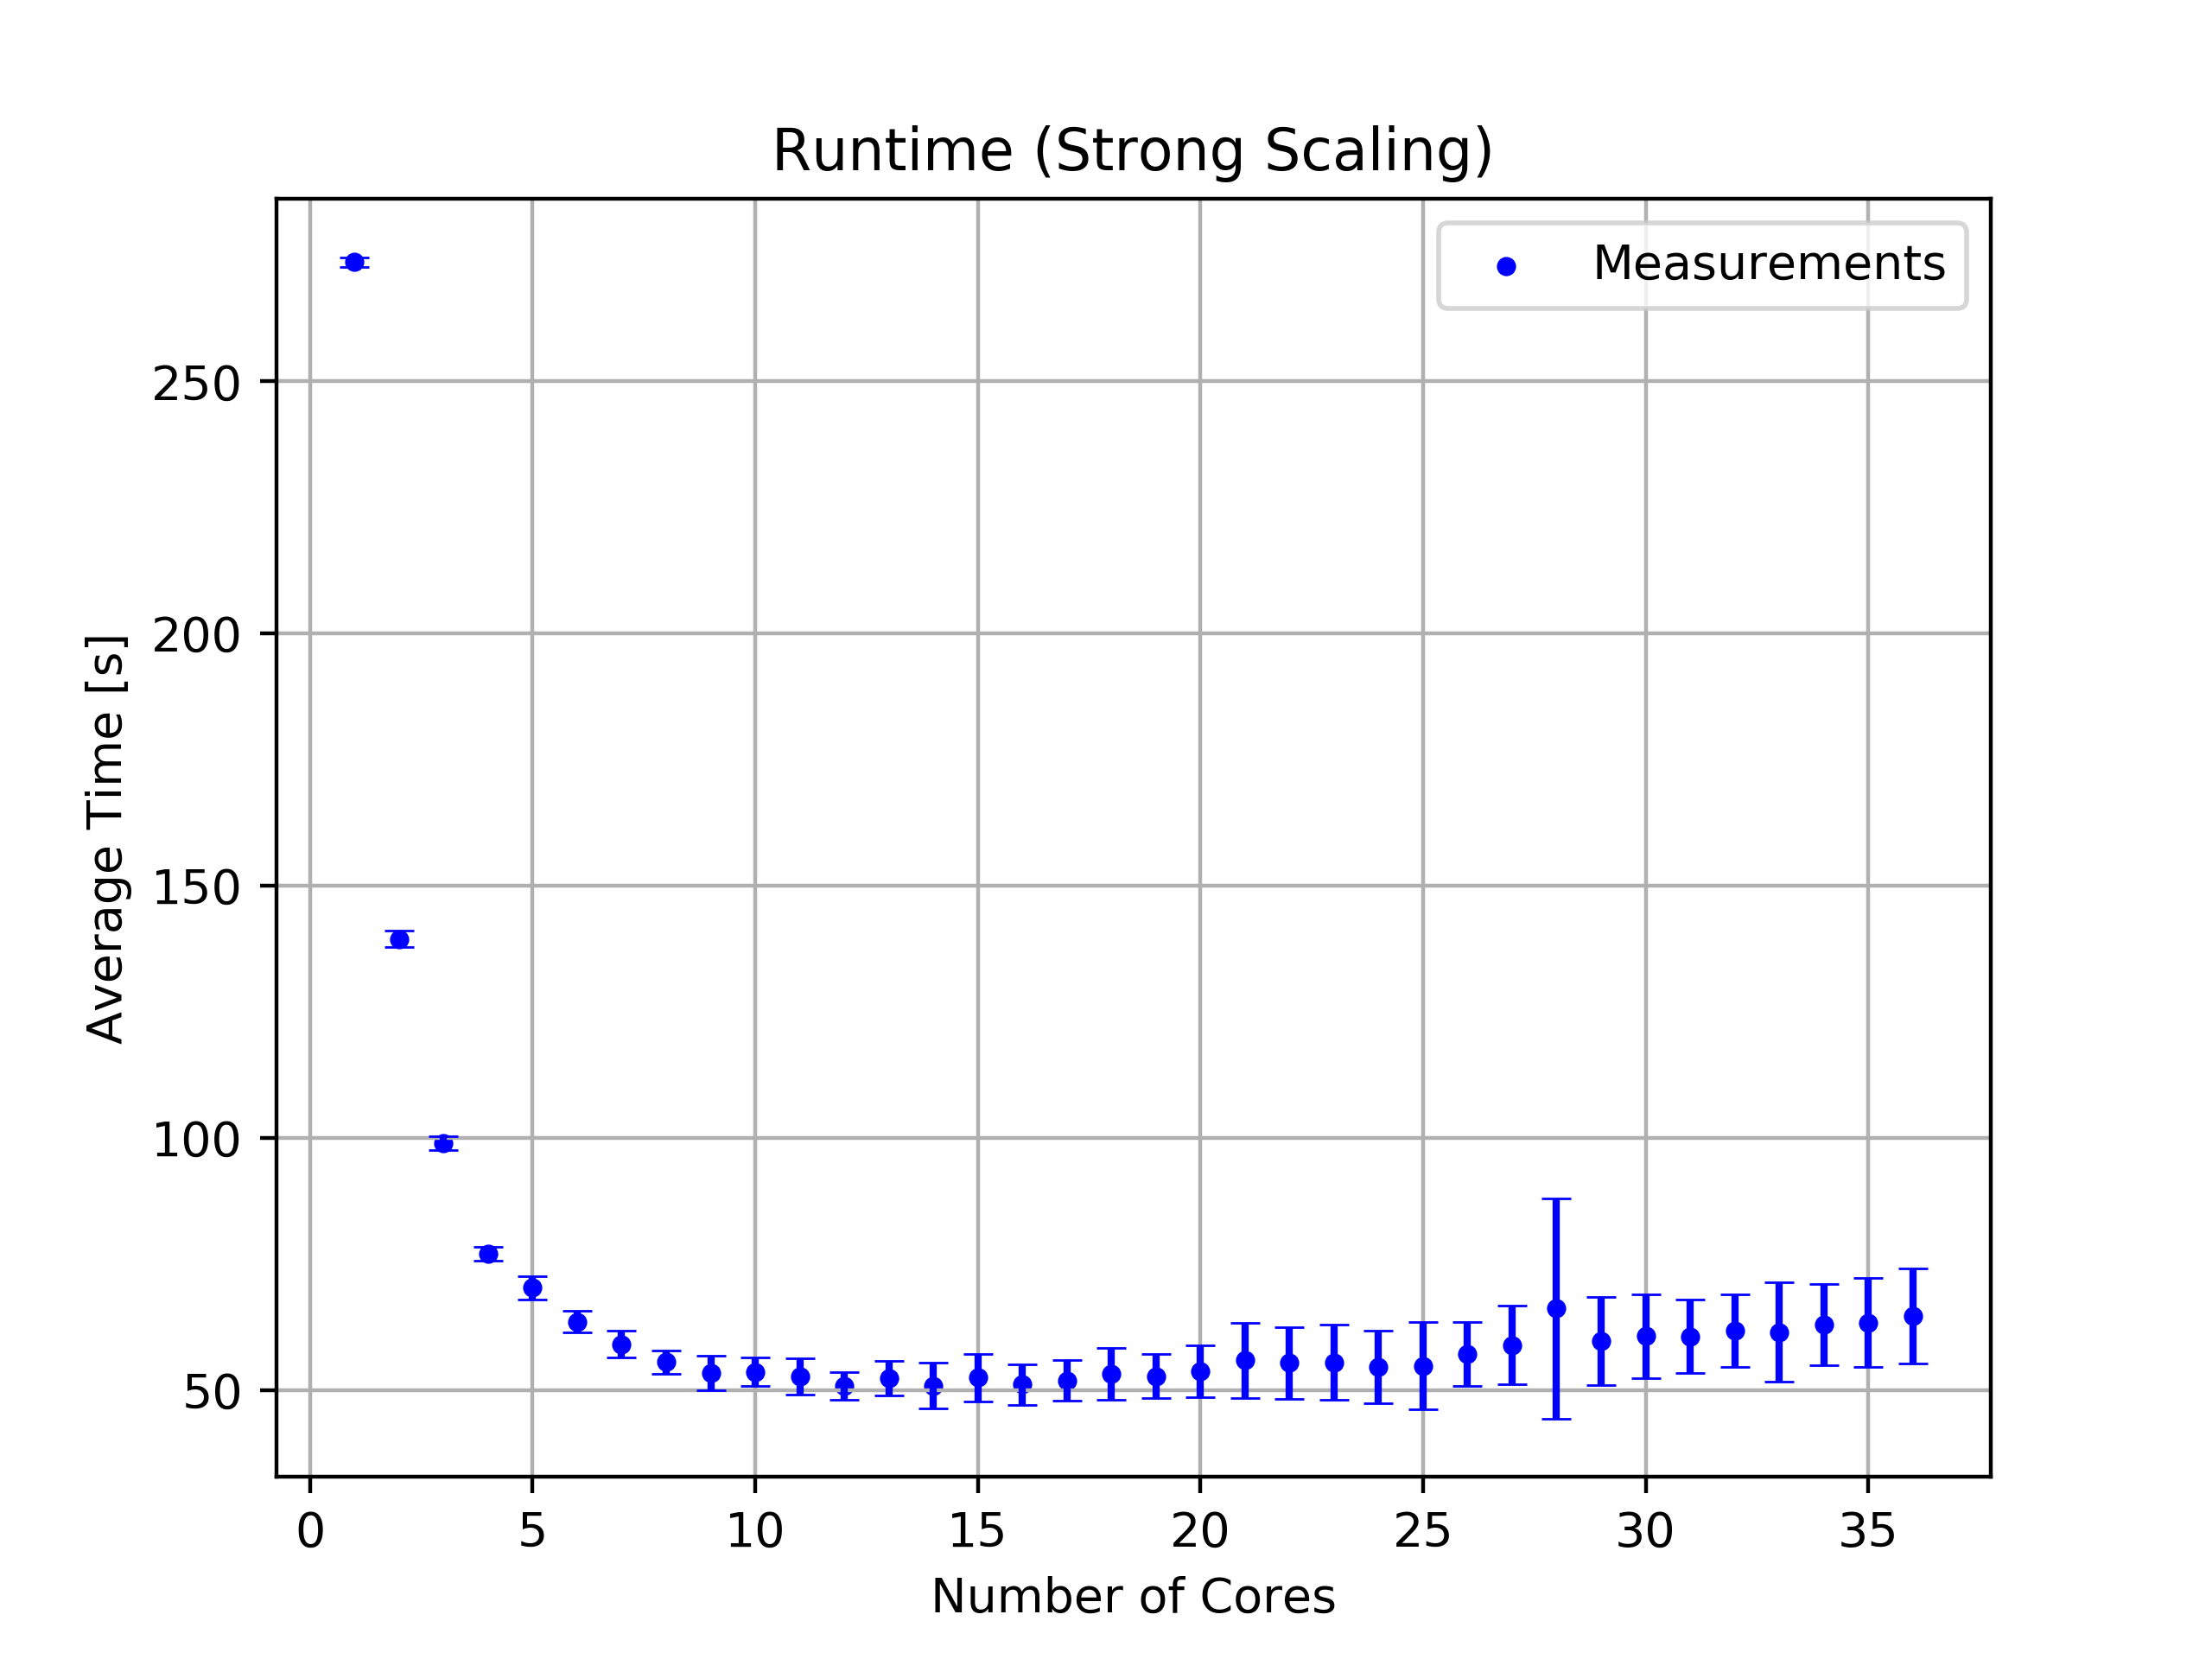
\includegraphics[width=\textwidth]{pictures/avg_strong.png}
	\end{minipage}
	\hfill
	\begin{minipage}{0.49\textwidth}
	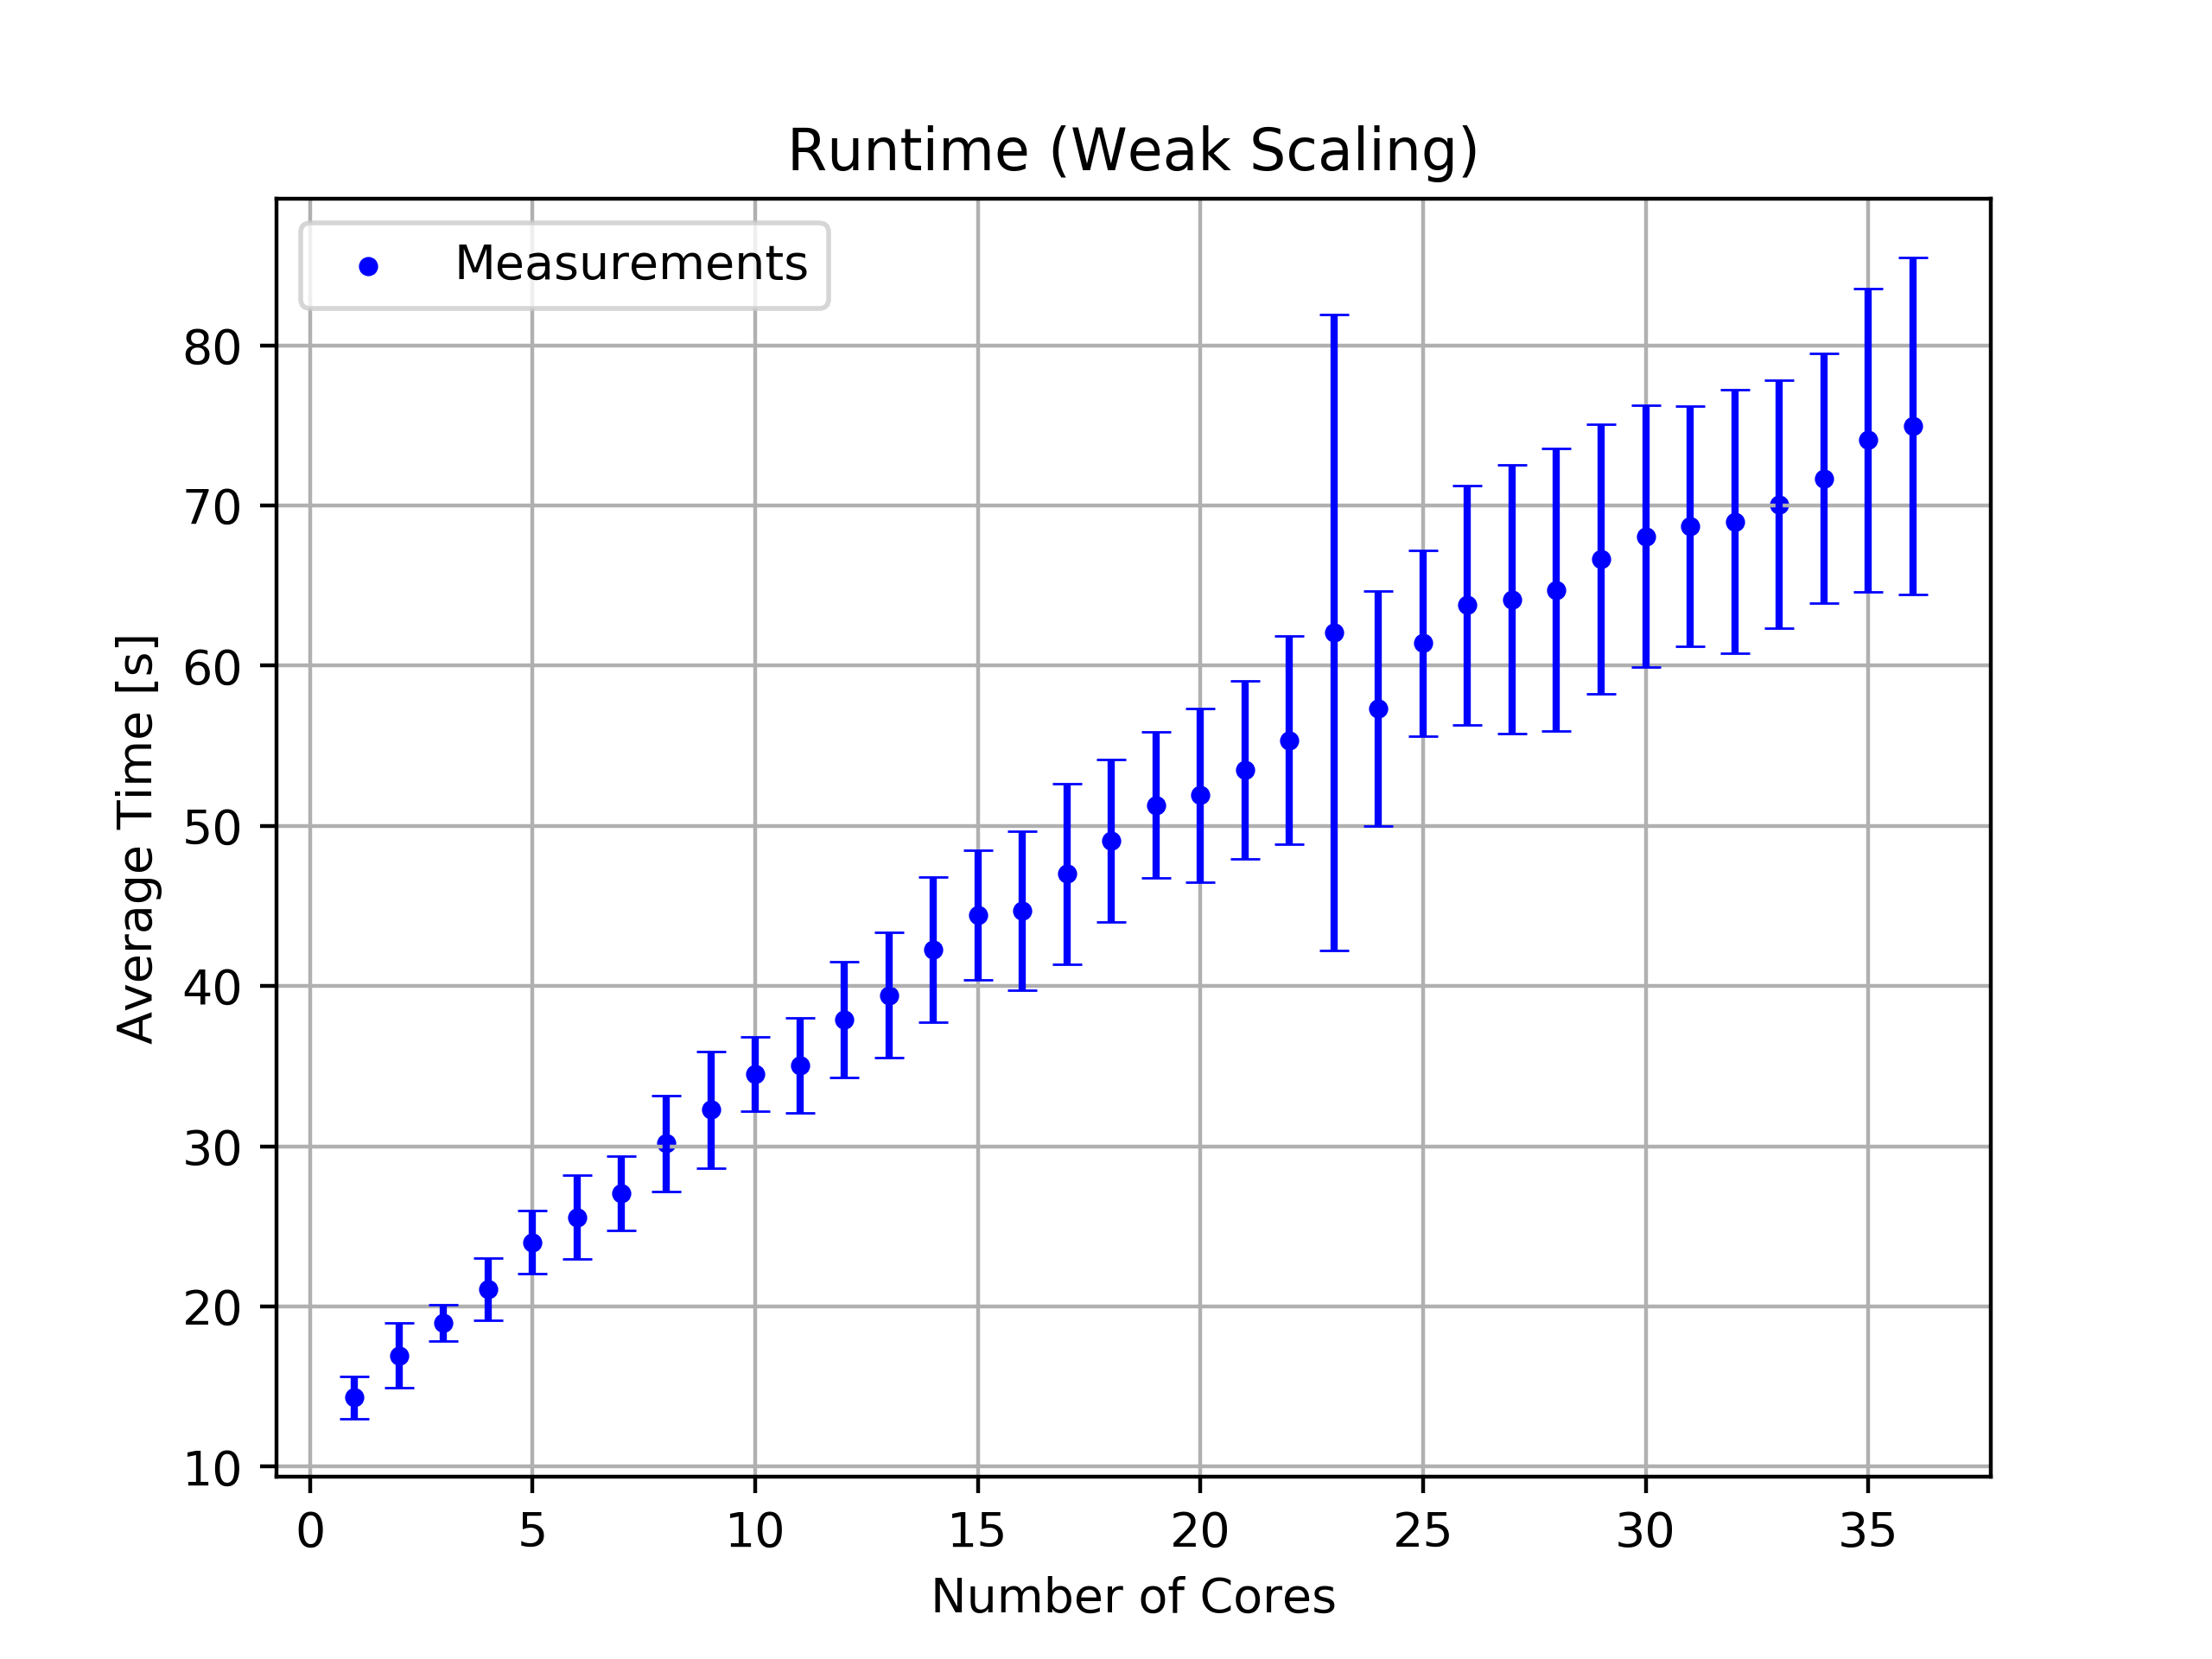
\includegraphics[width=\textwidth]{pictures/avg_weak.png}
	\end{minipage}
	\caption{Respective runtimes for strong and weak scaling}
	\label{fig:runtimes}
\end{figure}

The simulation was run from 1 to 36 cores 10 times each.

The settings for the strong scaling were the following:\\
\begin{center}
\begin{tabular}{c|c|c|c}
 $t_{\text{end}}$ & $nx$ & $ny$ & $\der x$ \\ \hline
 50.0 & 50 & 9000 & 0.08 \\
\end{tabular}
\end{center}

The settings for the weak scaling were the following:\\
\begin{center}
\begin{tabular}{c|c|c|c}
 $t_{\text{end}}$ & $nx$ & $ny$ & $\der x$ \\ \hline
 50.0 & 50 & 300 & 0.08 \\
\end{tabular}
\end{center}

Note that the $nx$ remained unchanged during the weak scaling run, but $ny$ increased linearly with the number of processes involved, $ny = ny \cdot $ (number of processes).


\begin{figure}[h!]
\begin{center}
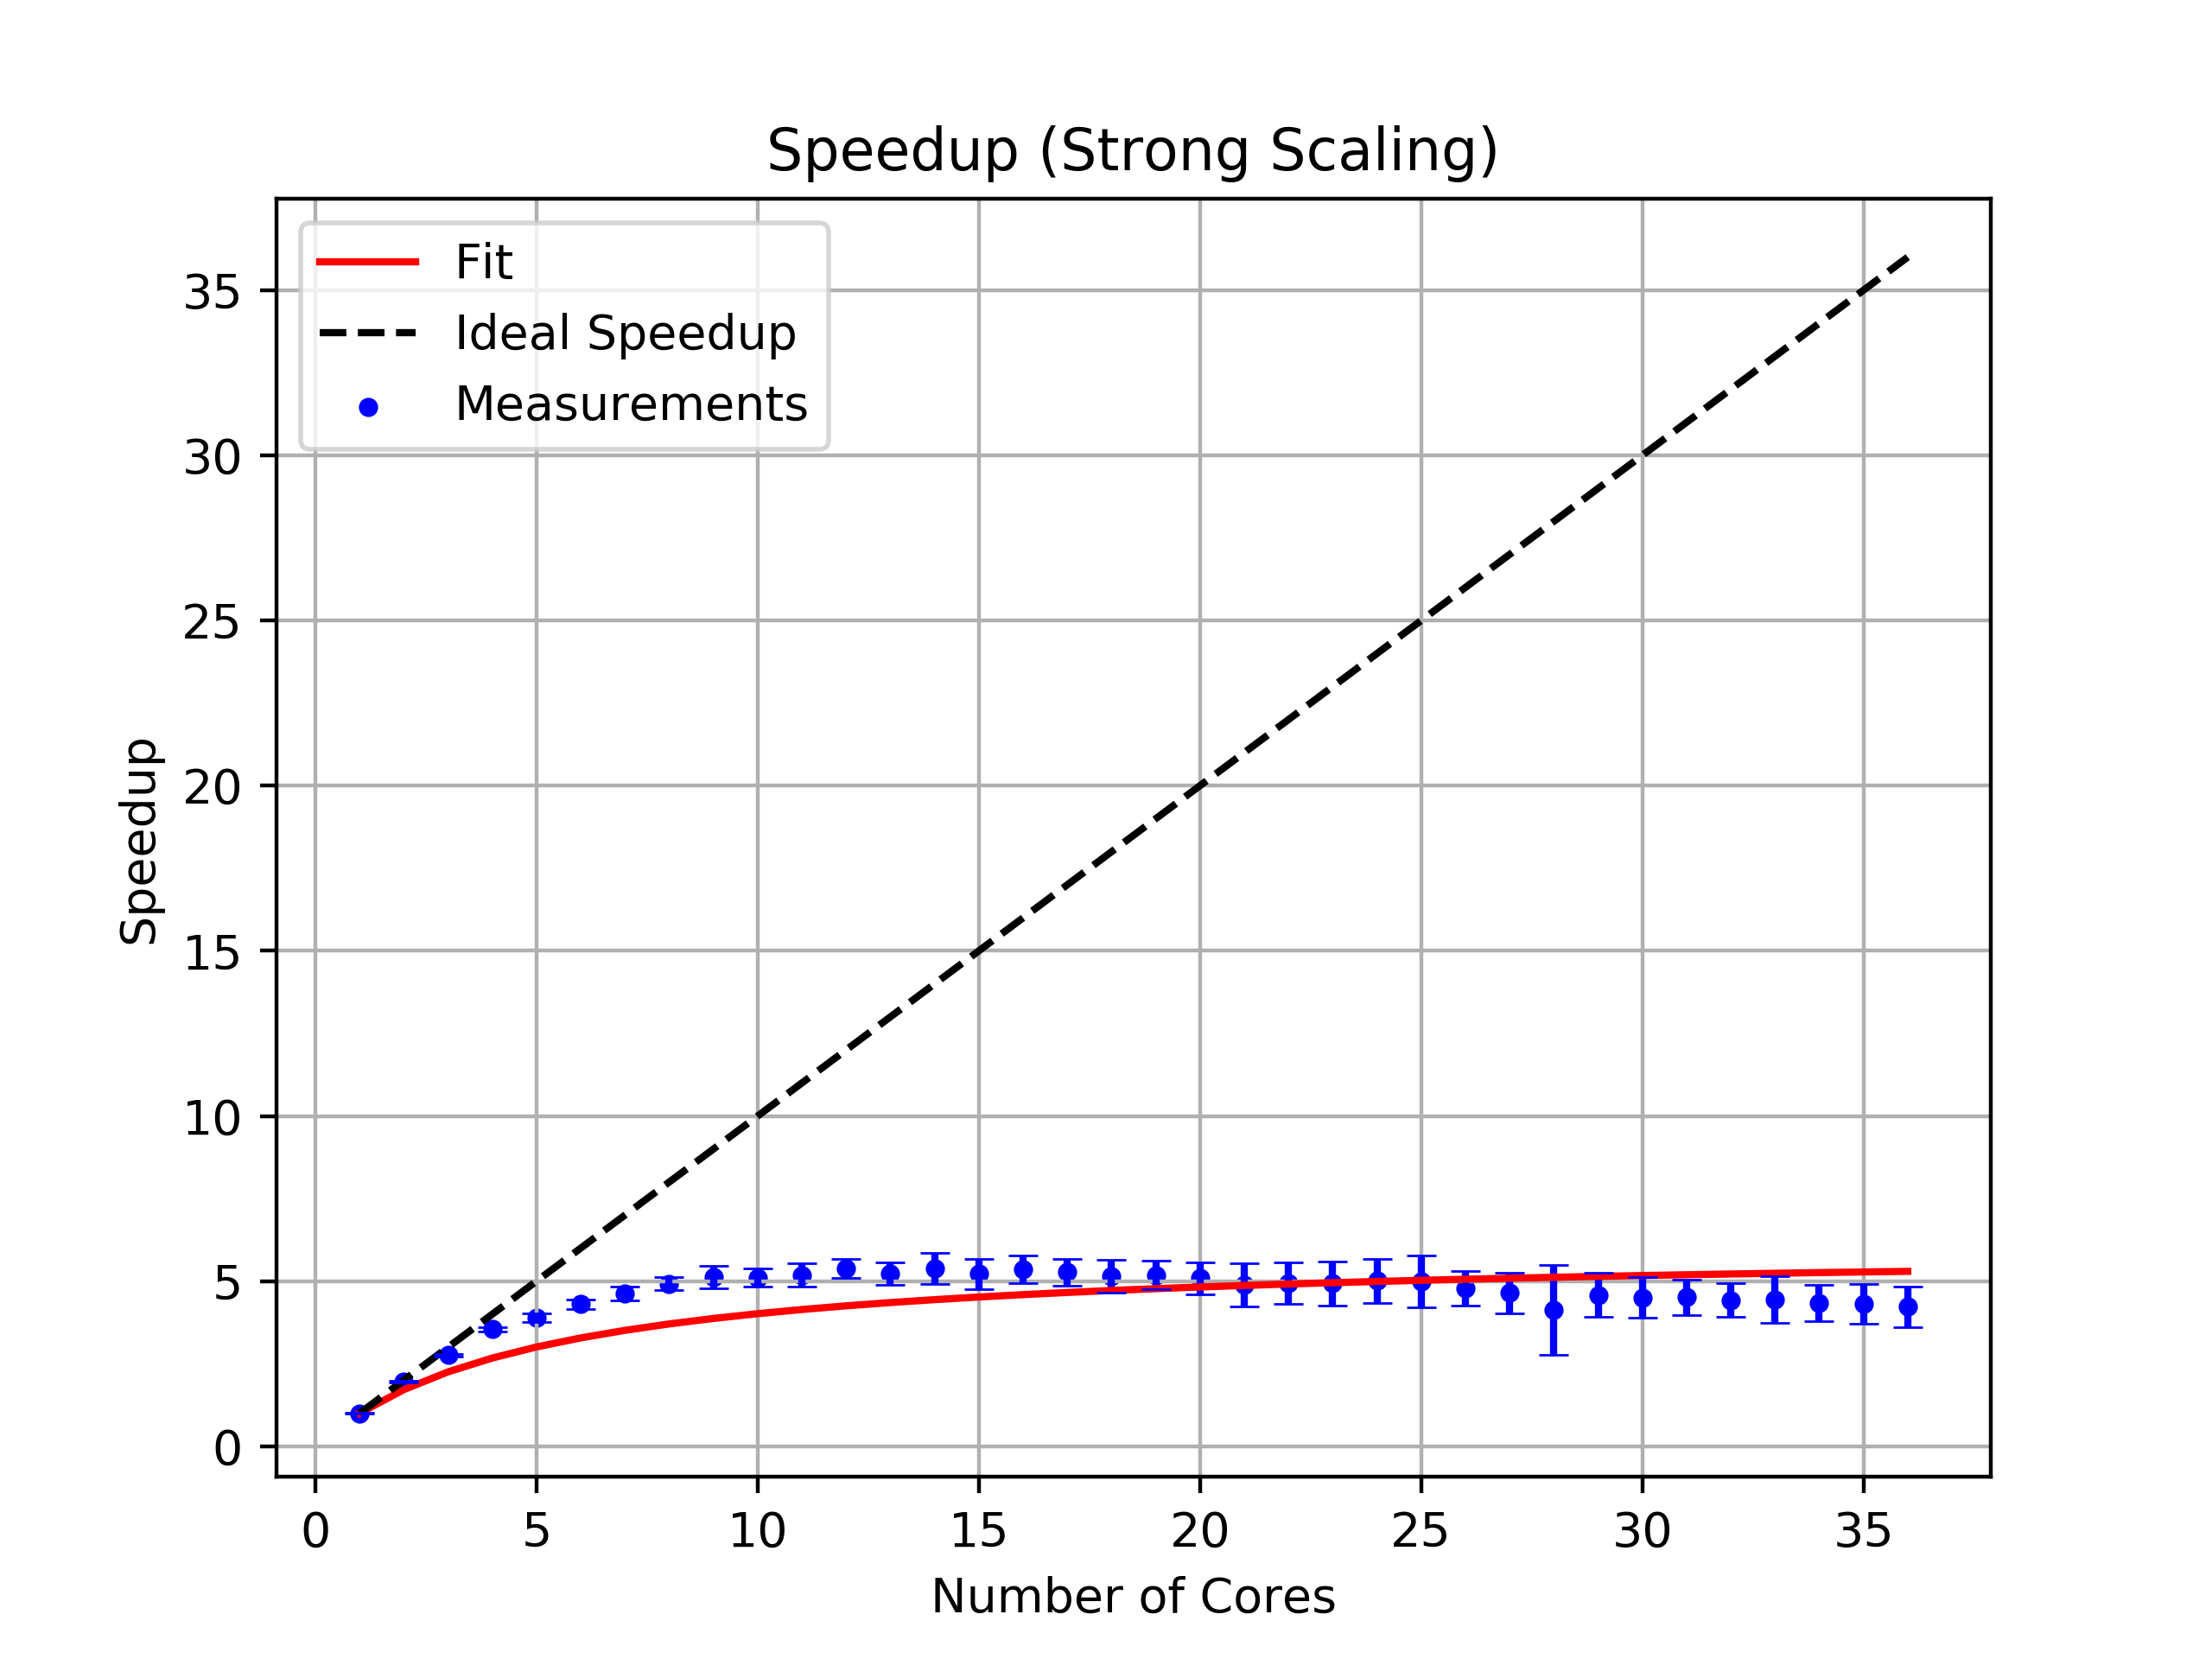
\includegraphics[width=0.8\textwidth]{pictures/speedup_strong.png}
\caption{Speedup for strong scaling}
\end{center}
\end{figure}


The fit for the strong scaling is done with the following formula (Lecture 5):
\begin{equation}
\frac{1}{\alpha + \frac{1-\alpha}{N}}
\end{equation}
Where $\alpha$ represents the non-parallelized fraction of the code, and $N$ is the number of processes.\\
This yields the following value:
\begin{equation} 
\alpha=
\end{equation}

\begin{figure}[h!]
\begin{center}
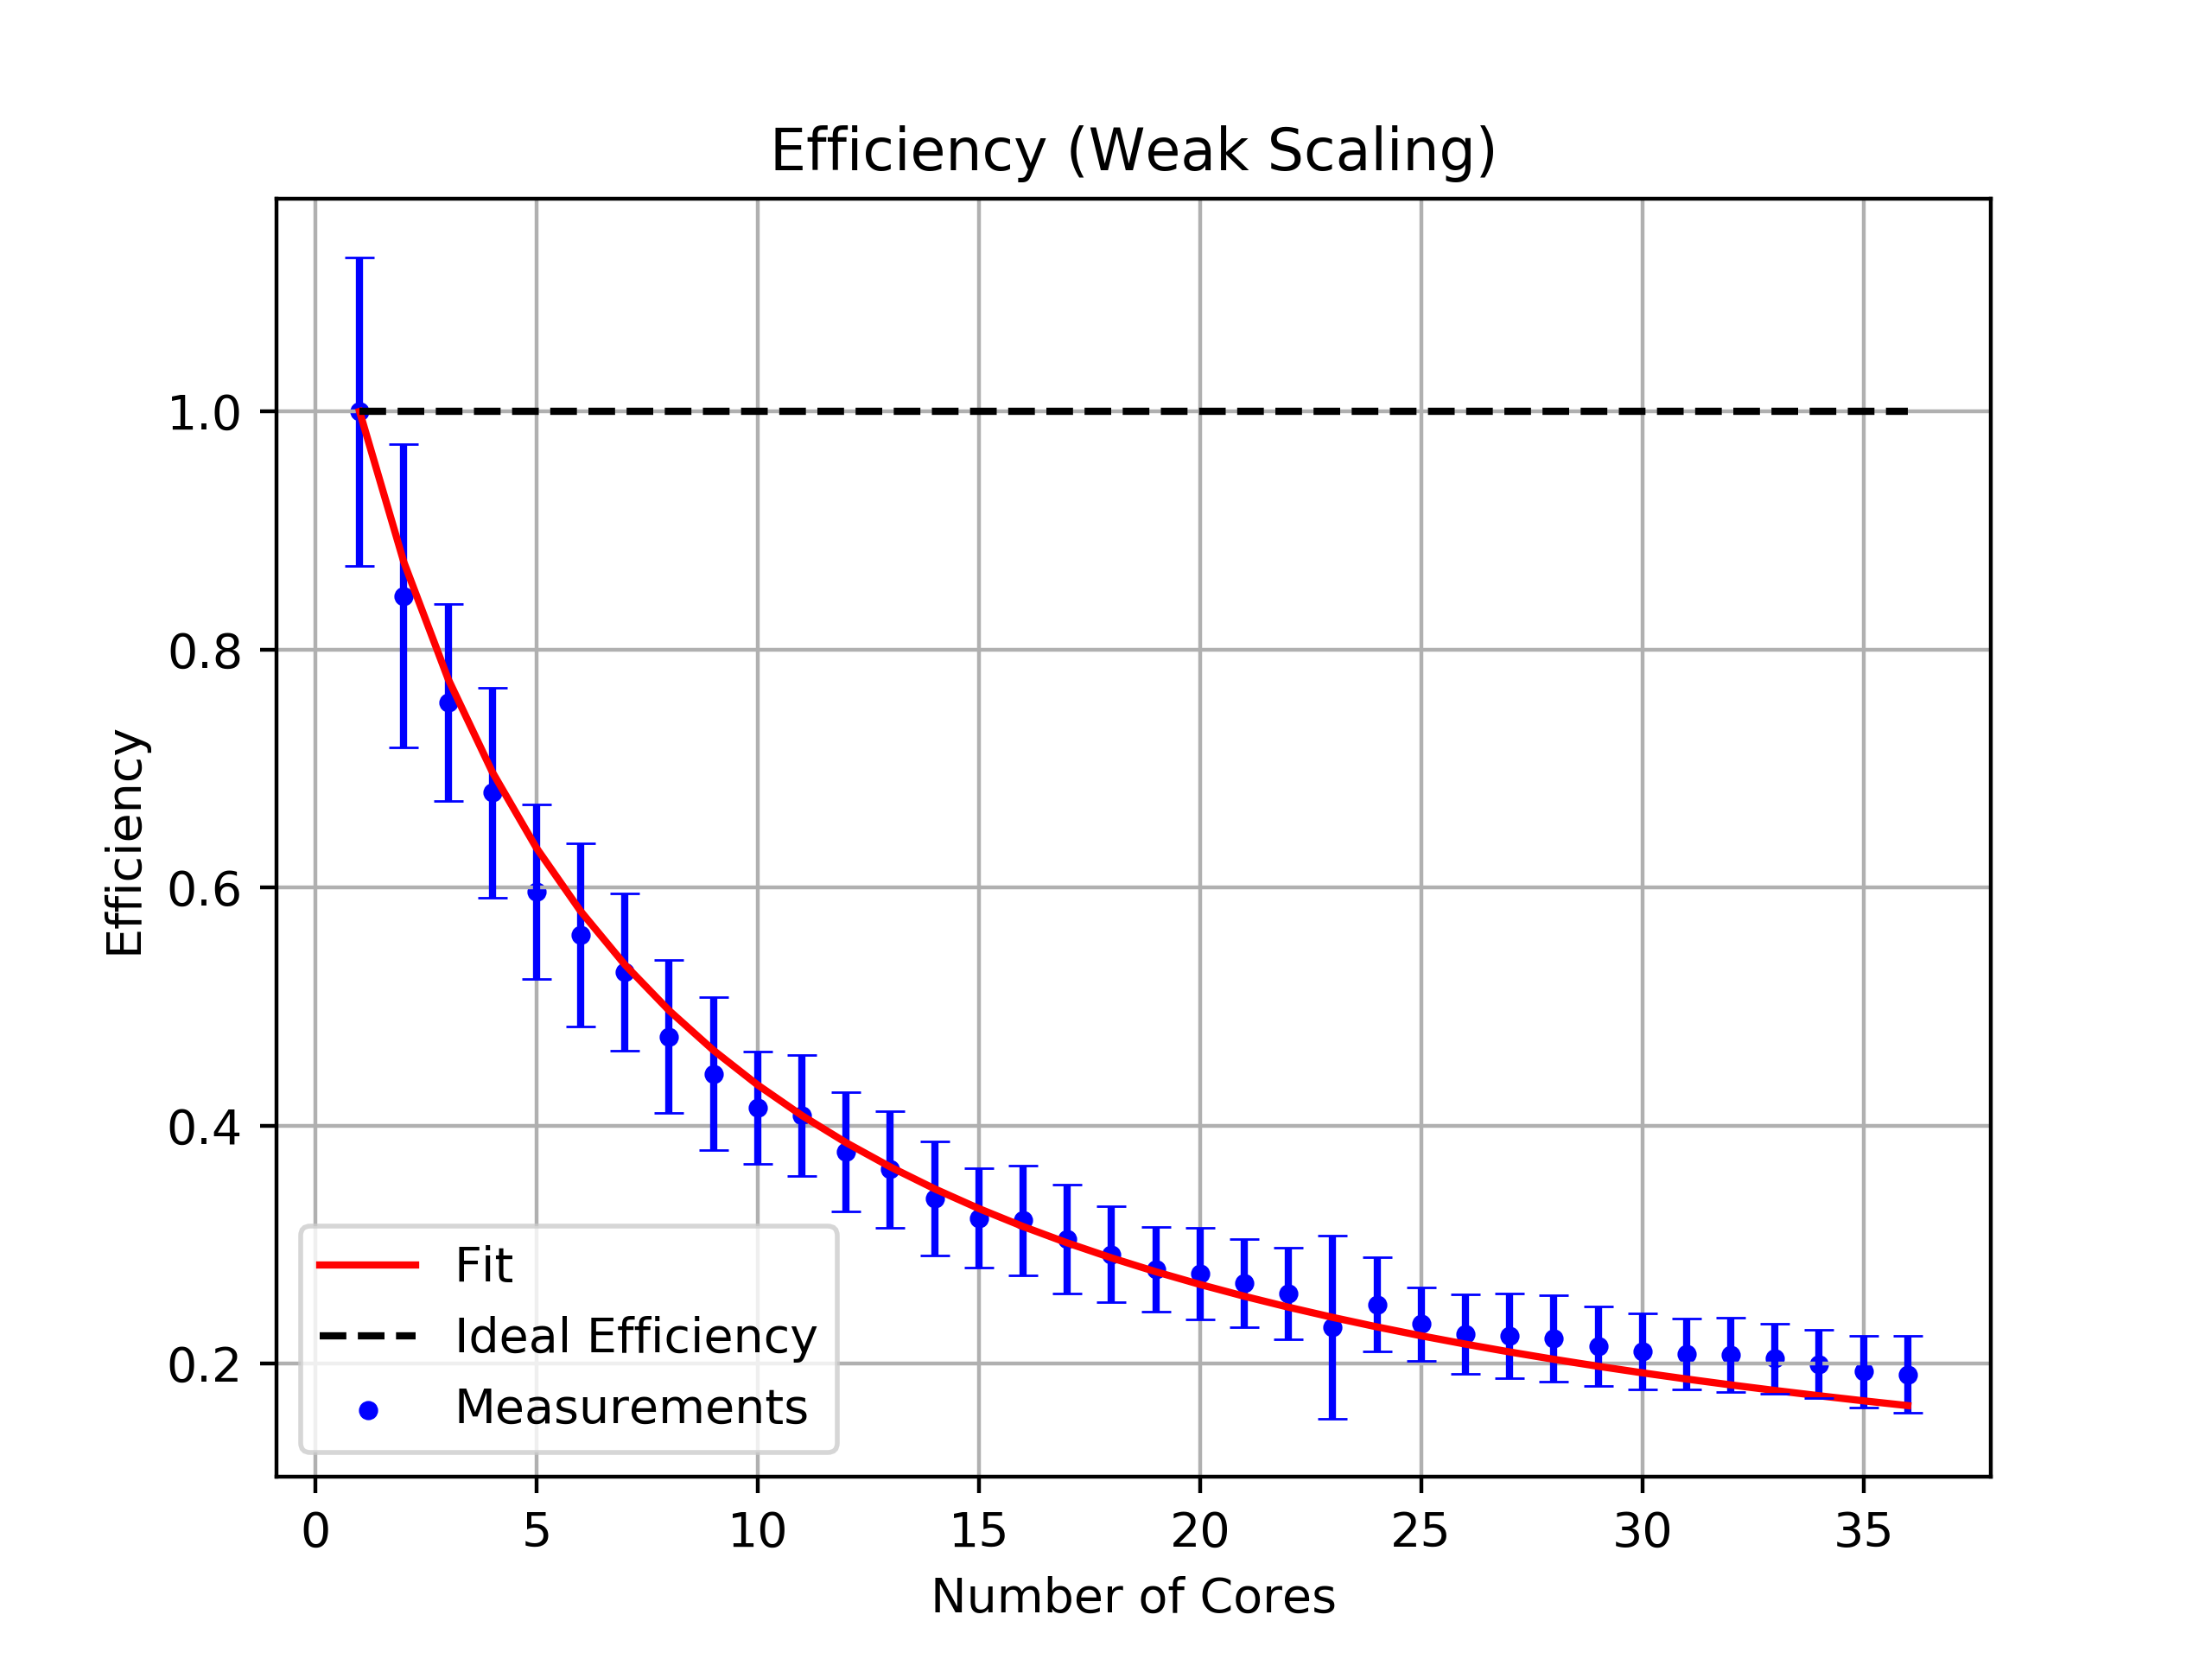
\includegraphics[width=0.8\textwidth]{pictures/speedup_weak.png}
\end{center}
\caption{Speedup for weak scaling}
\end{figure}
The formula for the fit for the weak scaling can be derived quite easily. Again, take $\alpha$ to be the non parallelized fraction of the code. Then, $T_p(N)$, the time needed for the parallel code, is\\
\begin{equation*}
T_p(N) = N \cdot (1 - \alpha) + \alpha
\end{equation*} 

So then, 
\begin{equation*}
\text{Speedup($N$)} = \frac{T_s(N)}{T_p(N)} = \frac{T_s}{T_p(N)} = \frac{1}{(1-\alpha)\cdot N + \alpha}
\end{equation*} 

Fitting this over the data yields:
\begin{equation}
\alpha = 
\end{equation}

\vp
\subsection{Other Techniques}

\subsubsection{OpenMP}


\subsubsection{MPI - OpenMP Hybrid}



\section{Discussion}

As can be seen in Figure \ref{fig:runtimes}, the standard deviation on some of the runtimes can be quite big. This is mainly due that the whole run (going from 1 to 36 precesses) was only performed 10 times. If one of these times is abnormally high or low, averaging over only 10 values will not suppress this spike well enough. 


\section{Conclusion}



\end{document}
